\documentclass{article}

\usepackage{graphicx}
\usepackage[utf8]{inputenc}
\usepackage[italian]{babel}
\usepackage{amsmath}

\begin{document}

\begin{titlepage}
\newcommand{\HRule}{\rule{\linewidth}{0.5mm}}
\center


\begin{figure}
\center

\includegraphics[scale=0.1]{logo}
\end{figure}


\textsc{\LARGE Università di Padova}\\[1.5cm]
\HRule \\[0.4cm]
{ \huge \bfseries Titolo}\\[0.4cm]
\HRule \\[1.5cm]

\begin{minipage}{0.4\textwidth}
\begin{flushleft} \large
\emph{Autori:}\\
Raffaele \textsc{La Torre} \\
Stefano \textsc{Campostrini}
\end{flushleft}
\end{minipage}
~
\begin{minipage}{0.4\textwidth}
\begin{flushright} \large
\emph{Supervisore:} \\
Prof.ssa Caterina \textsc{Braggio}
\end{flushright}
\end{minipage}\\[4cm]

{\large \today}\\[3cm]

\vfill
\end{titlepage}

\tableofcontents

\newpage
\begin{abstract}
Lo scopo dell'esperimento consiste nel determinare le lunghezze d'onda dello spettro di luce emessa dal Cadmio, utilizzando uno spettroscopio a reticolo di diffrazione. \\
Noto il passo $d$ del reticolo e misurato all'ordine $m$ l'angolo di diffrazione $sin\theta_{m}$ relativo a tale ordine, la lunghezza d'onda è data dall'equazione del reticolo: 

\begin{equation}
\lambda =  \frac{d sin\theta_m}{m}
\end{equation}

Le lunghezze d'onda dello spettro del Cadmio sono note, e sono riassunte in Tab.1. 

\begin{center}
 \begin{tabular}{|c|c|}
   \hline
   $\lambda$ $(nm)$ & colore \\ \hline
   441.6 & violetto \\
   467.8 & blu \\
   480.0 & azzurro \\
   508.6 & verde \\
   643.8 & rosso \\ \hline
 \end{tabular}
\end{center}

\end{abstract}

\newpage
\section{Apparato sperimentale}

L'apparato sperimentale consiste in uno spettroscopio, schematizzato in Fig.1. \\
Una struttura cilindrica supporta un tavolo rotante coassiale che porta il reticolo. Dal supporto si protendono due bracci: uno viene fissato rigidamente al supporto e porta un collimatore con una fenditura di apertura variabile; sul secondo braccio è montato un telescopio che riceve la luce dal reticolo. Il ramo su cui è montato il telescopio può ruotare indipendentemente attorno all`asse centrale, per la ricerca di una particolare componente spettrale, e porta una scala graduata (interna) che si muove rispetto ad una scala graduata esterna. Sono presenti due zone sulla scala graduata, diametralmente opposte, che permettono di effettuare la misura; questo per limitare gli errori dovuti all'eccentricità.


\begin{figure}[!ht]
\center
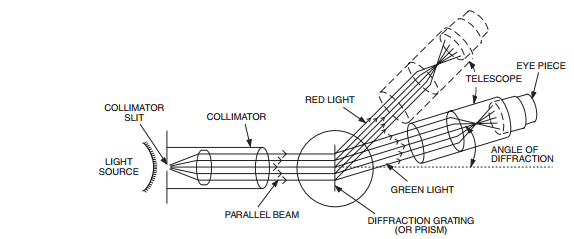
\includegraphics[scale=0.8]{spettroscopio2}
\end{figure}

Il passo del reticolo è: 
\begin{center}
$d = (12.650 \pm 0.05)\mu m$
\end{center}

L'errore sistematico sulla lettura dell'angolo è $\Delta\theta = 0^{\circ} 02'$. \\


\newpage
\section{Procedura}
La procedura è divisa nelle seguenti fasi: \\

\begin{enumerate}
\item Allineamento dello spettroscopio. Il reticolo di diffrazione deve essere allineato con l'asse ottico del telescopio e del collimatore. Per posizionare il reticolo ortogonalmente all'asse ottico si procede nel modo seguente:

\end{enumerate}

\newpage
\section{Raccolta dati}
 

\newpage
\section{Elaborazione dati}
 

\newpage
\section{Conclusioni}














\end{document}
